\documentclass[dsc,numbers]{coppe}
\usepackage[utf8]{inputenc}
\usepackage{amsmath,amssymb}
\usepackage{hyperref}

\makelosymbols
\makeloabbreviations

\begin{document}
  \title{Título da Tese}
  \foreigntitle{Thesis Title}
  \author{Nome do Autor}{Sobrenome}
  \advisor{Prof.}{Nome do Primeiro Orientador}{Sobrenome}{D.Sc.}
  \advisor{Prof.}{Nome do Segundo Orientador}{Sobrenome}{Ph.D.}
  \advisor{Prof.}{Nome do Terceiro Orientador}{Sobrenome}{D.Sc.}

  \examiner{Prof.}{Nome do Primeiro Examinador Sobrenome}{D.Sc.}
  \examiner{Prof.}{Nome do Segundo Examinador Sobrenome}{Ph.D.}
  \examiner{Prof.}{Nome do Terceiro Examinador Sobrenome}{D.Sc.}
  \examiner{Prof.}{Nome do Quarto Examinador Sobrenome}{Ph.D.}
  \examiner{Prof.}{Nome do Quinto Examinador Sobrenome}{Ph.D.}
  \department{PEC}
  \date{02}{2011}

  \keyword{Primeira palavra-chave}
  \keyword{Segunda palavra-chave}
  \keyword{Terceira palavra-chave}

  \maketitle

  \frontmatter
  \dedication{À minha mãe pelo dom da vida e pelo amparo ao longo desses anos.\\
Às minhas tias Vanete e Vanilde (\emph{in memoriam}).}


  \chapter*{Agradecimentos}

Gostaria de agradecer a todos.

  \begin{abstract}

Autovalores e autovetores de operadores lineares são importantes para muitas
áreas da Matemática Aplicada. Na Engenharia Civil, sobretudo na Engenharia de
Estruturas o uso de problemas de autovalor tem fundamental importância, um
exemplo típico é a análise dinâmica, onde os autovalores representam as
frequências naturais e os autovetores os modos de vibração associados à sua
frequência natural correspondente. A crescente demanda da avaliação numérica de
forma mais eficiente dessas quantidades, despertou o interesse na busca de
novos métodos para a solução de problemas de autovalor, principalmente quando o
problema a ser analisado conduz a quantidades pertencentes ao conjunto dos
números complexos.

\end{abstract}


  \begin{foreignabstract}

Eigenvalues and eigenvectors of linear operators are important in many Applied
Mathematics areas. In Civil Engineering, especially in Structural Analysis,
eigensystems have a fundamental importance. A typical example is in dynamic
analysis, where the eigenvalues represent the natural frequencies and
eigenvectors the mode shape. The increasing demand for efficient numeric
evaluation of eigenvalues and eigenvectors motivated the search for new methods
for the solution of complex eigensystems.

\end{foreignabstract}


  \tableofcontents
  \listoffigures
  \listoftables
  \printlosymbols
  \printloabbreviations

  \mainmatter
  \chapter{Introdução}

Em métodos numéricos para obter soluções aproximadas de equações diferenciais,
tais como o método dos elementos finitos (MEF) e o método dos volumes finitos
(MVF), o domínio no qual estas equações foram definidas é discretizado em
sub-domínios simples denominados \textit{elementos}.%
\abbrev{MEF}{método dos elementos finitos}%
\abbrev{MVF}{método dos volumes finitos}

Denotemos o domínio por $\Omega$. Seja $\partial \Omega$ o contorno de
$\Omega$.%
\symbl{$\Omega$}{domínio de definição de uma equação diferencial}%
\symbl{$\partial$}{operador do contorno}

\section{Motivaç{\~ a}o}

\section{Objetivo}

\section{Metodologia}

\section{Organizaç{\~ a}o da tese}

  \chapter{Revisão Bibliográfica}

Para ilustrar a completa ades\~ao ao estilo de cita{\c c}\~oes e listagem de
refer\^encias bibliogr\'aficas, a Tabela~\ref{tab:citation} apresenta cita{\c
c}\~oes de alguns dos trabalhos contidos na norma fornecida pela CPGP da
COPPE, utilizando o estilo num\'erico.

\begin{table}[h]
\caption{Exemplos de cita{\c c}\~oes utilizando o comando padr\~ao
  \texttt{\textbackslash cite} do \LaTeX\ e
  o comando \texttt{\textbackslash citet},
  fornecido pelo pacote \texttt{natbib}.}
\label{tab:citation}
\centering
{\footnotesize
\begin{tabular}{|c|c|c|}
  \hline
  Tipo da Publica{\c c}\~ao & \verb|\cite| & \verb|\citet|\\
  \hline
  Livro & \cite{book-example} & \citet{book-example}\\
  Artigo & \cite{article-example} & \citet{article-example}\\
  Relat\'orio & \cite{techreport-example} & \citet{techreport-example}\\
  Relat\'orio & \cite{techreport-exampleIn} & \citet{techreport-exampleIn}\\
  Anais de Congresso & \cite{inproceedings-example} &
    \citet{inproceedings-example}\\
  S\'eries & \cite{incollection-example} & \citet{incollection-example}\\
  Em Livro & \cite{inbook-example} & \citet{inbook-example}\\
  Disserta{\c c}\~ao de mestrado & \cite{mastersthesis-example} &
    \citet{mastersthesis-example}\\
  Tese de doutorado & \cite{phdthesis-example} & \citet{phdthesis-example}\\
  \hline
\end{tabular}}
\end{table}


  \chapter{M�todo Proposto}

\section{O Algoritmo}

\begin{figure}[b]
\centering
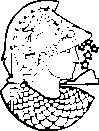
\includegraphics{minerva}
\caption{Deusa Minerva.}
\label{fig:minerva}
\end{figure}

  \chapter{Resultados e Discussões}

\section{Metodologia para avaliaç{\~ a}o do M{\' e}todo}

\section{Validaç{\~ a}o da rotina implementada}

\subsection{Problema de autovalor padr{\~ a}o -- Caso I}

A Tabela~\ref{table:casoi} mostra as variações dos parâmetros escolhidos para
análise.

\begin{table}[b]
\caption{Par{\^ a}metros do teste realizado com a matriz de Wilkinson,
3 autovalores computados.}
\label{table:casoi}
\centering
\begin{tabular}{cccc}
  \hline
  Valor de ``m'' & N$^{o}$ de iteraç{\~ o}es & Tempo de CPU & Norma do Res{\' i}duo\\
  \hline
  6 & 100 & 0,09013 & $7,1474 \times 10^{-12}$\\
  10 & 28 & 0,09025 & $1,5387 \times 10^{-13}$\\
  20 & 10 & 0,100144 & $5,9011 \times 10^{-14}$\\
  40 & 6 & 0,16022 & $8,67438 \times 10^{-14}$\\
  50 & 3 & 0,24034 & $1,51537 \times 10^{-15}$\\
  \hline
\end{tabular}
\end{table}

  \chapter{Conclusões}


  \backmatter
  \bibliographystyle{coppe-unsrt}
  \bibliography{thesis}

  \appendix
  \chapter{Código Fonte}
\end{document}
